\documentclass{article}
\usepackage[left=3cm, right=3cm, top=2cm]{geometry}
\usepackage{amsmath}
\usepackage{amsfonts}
\usepackage{graphicx}
\usepackage{color}
\title{A Small \LaTeX{} Article Template\thanks{To your mother}}
\author{Your Name  \\
	Your Company / University  \\
	\and 
	The Other Dude \\
	His Company / University \\
	}

\date{\today}
% Hint: \title{what ever}, \author{who care} and \date{when ever} could stand 
% before or after the \begin{document} command 
% BUT the \maketitle command MUST come AFTER the \begin{document} command! 
\begin{document}
\vspace{-10pt}
In response to Comments 1-3 from \underline{Reviewer: 5 (Review30371)} following we mathematically and graphically analyze the proposed local behavior synergy extraction scheme which is composed of dimensionality reduction of the joint trajectories (via. PCA or K-PCA) and grouping of local behavior regions with GMM on this lower dimensional space. The $K$ clusters found in this embedded space correspond to the number of $K$ synergy matrices that will parametrize $\mathcal{A}(q)$. Let's begin by analyzing the proposed DS-based control-law:
\begin{equation}
\underbrace{\dot{q}}_{\mathbb{R}^{m\times 1}} = -\underbrace{\mathcal{A}(q)}_{\mathbb{R}^{m\times m}}\underbrace{J^{T}(q)}_{\mathbb{R}^{m\times d}}\underbrace{(H(q)-x^*)}_{\mathbb{R}^{d\times 1}}
\label{eq:jtds}
\end{equation}
The intuition behind this control-law is that $\mathcal{A}(q) = \sum\limits_{k=1}^{K}\theta(\phi(q))A_k$ is a linear combination of time-invariant linear matrices $A_k \in \mathbb{R}^{m \times m}$, \underline{these matrices are the ``local behavior synergy matrices"} that shape the motion in joint-space. Meaning that, given the joint-space velocity vector representing the task-space error $J^{T}(q)(H(q)-x^*)$, the resulting motion is biased to use a particular set of joints, defined in each $A_k$. Each $A_k$ is thus activated depending on the current ``joint-posture" $q$ (represented in the lower-dimensional space $\phi(q)$) via the scheduling/activation function $\theta(\phi(q))$. Hence, our proposed definition of ``local behavior synergies" is \underline{not analogous} to the notion of ``hand posture synergies". 

Given the raw demonstrations of a joint-space  behavior with a task-space target as shown in Fig. \ref{fig:raw_demos} (for the pouring task) we seek to learn a linear combination of local behavior synergies $\mathcal{A}(q) = \sum\limits_{k=1}^{K}\theta(\phi(q))A_k$ such that we can use \eqref{eq:jtds} to accurately reproduce these demonstrations. In order to do so, we project the raw joint trajectories to a lower-dimensional space via $\phi(q)$, in the case of PCA $\phi(q)=M_p \times q$ for $M_p \in \mathbb{R}^{p \times m}$. By choosing the first 3 PCs we can explain 95\% of the variance in the joint posture trajectories, which can be represented in this 3-D space as shown in Fig. \ref{fig:raw_demos}. We then jointly learn the activation function $\theta(\cdot)$ and the number of $K$ local synergy regions by fitting a GMM to this representation of the joint posture trajectories. As can be seen in Fig. \ref{fig:raw_demos}, the entire joint-space motion can be represented by 3 local synergy regions in PCA-space. Meaning that we only need 3 synergy matrices $A_k$ to represent the complex joint-space motion accurately. The activation function $\theta(\cdot)$, as described in the mansucript, is the posterior probability of a joint posture in PCA-space $\phi(q)$ belonging to one of the local synergy regions $k \in \{1,\dots,K\}$.


\begin{figure*}[!th] 
  \begin{minipage}{0.58\textwidth}
     	\centering 
     	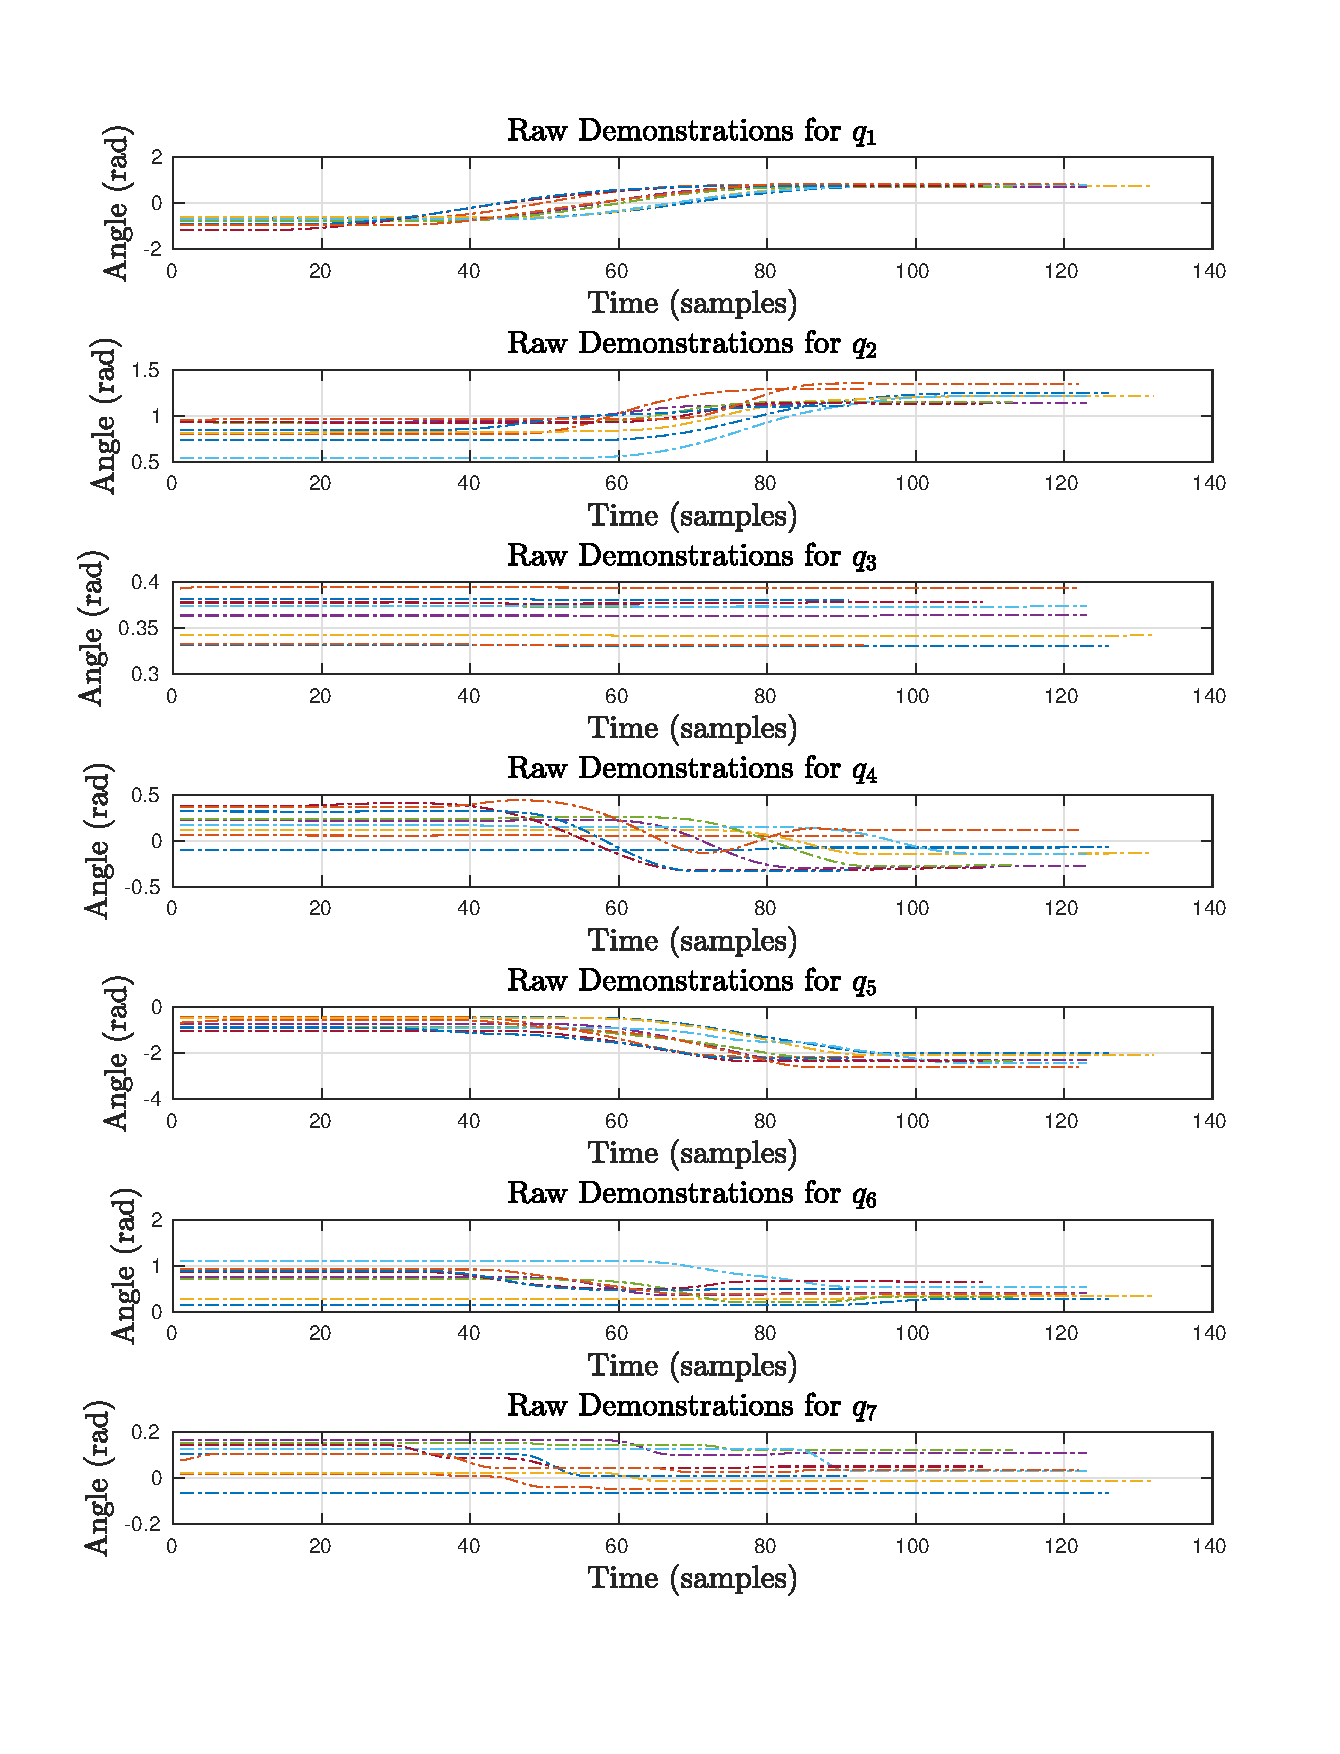
\includegraphics[trim={1.2cm 2cm 1.7cm 2cm},clip,width=\linewidth]{../../src/JTDS_mat_lib/figures/raw_demos_pour.pdf}
  \end{minipage}
   \begin{minipage}{0.47\textwidth}
      	\centering
      	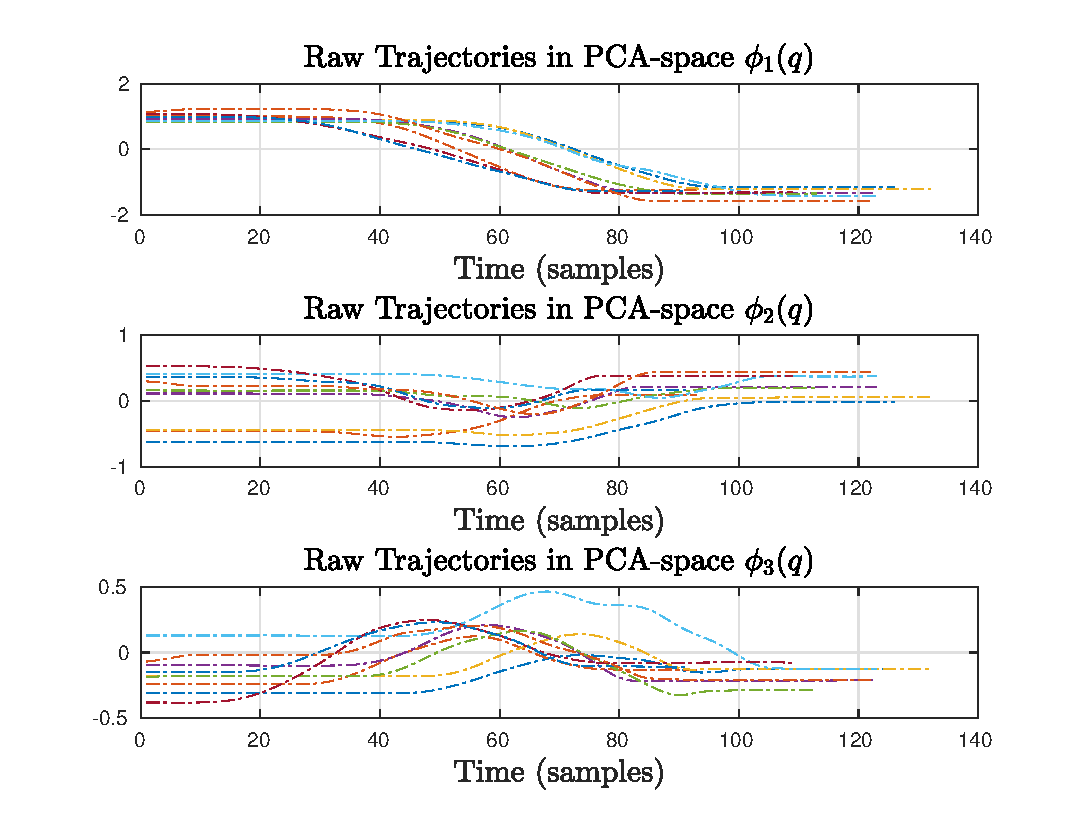
\includegraphics[trim={1.2cm 0.5cm 0.5cm 0.35cm},clip,width=\linewidth]{../../src/JTDS_mat_lib/figures/raw_demos_pca_pour.pdf}
      	\vspace{-5pt}
      	
		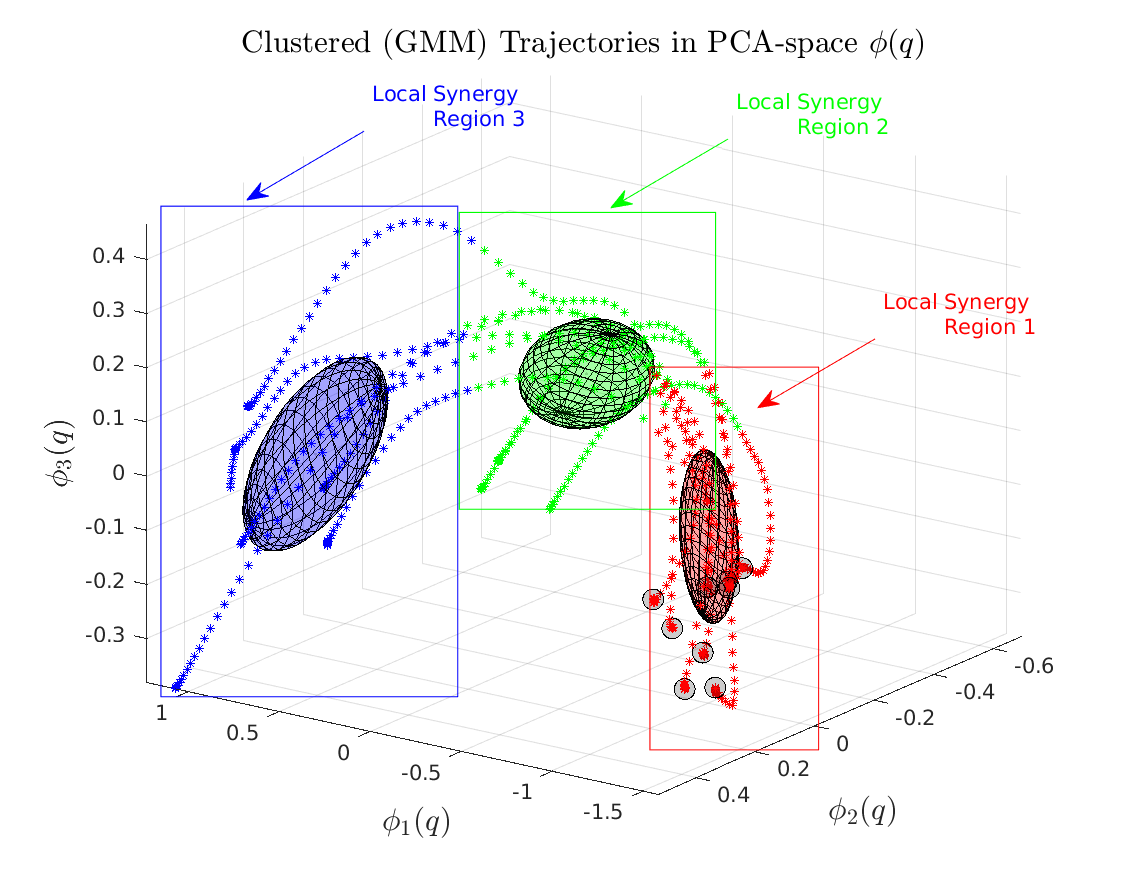
\includegraphics[trim={0.8cm 0.5cm 0cm 0.35cm},clip,width=\linewidth]{../../src/JTDS_mat_lib/figures/local_synergy_regions_pour_annotated.pdf}
   \end{minipage}
   \caption{Raw demonstrations of the pouring task in original space, PCA space and the extracted local synergy regions. \label{fig:raw_demos}}
\end{figure*}

\underline{As mentioned in the reviewers 3rd comment}, since we have an accurate representation of our joint posture trajectories and the local synergy regions in this lower-dimensional space, why not learn the $A_k$ matrices in this space; i.e. $\mathcal{A}(q)\in \mathbb{R}^{p\times p}$ rather than $\mathcal{A}(q)\in \mathbb{R}^{m\times m}$ ? This seems like the obvious method, if we were considering our synergistic approach the classical way, i.e. using the lower-dimensional space as the new control variables. However, if we were to do that, this would mean that \eqref{eq:jtds} would become:
\begin{equation}
\underbrace{\dot{q}}_{\mathbb{R}^{m\times 1}} = -\underbrace{M_p^{-1}}_{\mathbb{R}^{m\times p}}\underbrace{\mathcal{A}(q)}_{\mathbb{R}^{p\times p}}\underbrace{M_p}_{\mathbb{R}^{p\times m}}\underbrace{J^{T}(q)}_{\mathbb{R}^{m\times d}}\underbrace{(H(q)-x^*)}_{\mathbb{R}^{d\times 1}}
\label{eq:jtds_low}
\end{equation}
This is not entirely incorrect, however, with such a control law we can no longer guarantee stability and convergence to the attractor $x^{*}$. By considering the Lyapunov function used in Appendix I to prove stability of \eqref{eq:jtds_low} i.e. $V(q) = \frac{1}{2}(H(q) - x^*)^T(H(q) - x^*)$, the derivative of $ V $ wrt. would be:
\begin{equation}
\begin{aligned}
\frac{dV(q)}{dt} &= (H(q) - x^*)^TJ(q)\dot{q}\\
&= -(H(q) - x^*)^TJ(q)M_p^{-1}\mathcal{A}(q)M_pJ^T(q)(H(q) - x^*)\\
&= -(H(q) - x^*)^TJ(q)\textcolor{red}{\underbrace{M_p^{-1}\big(\sum_{k=1}^{K}\underbrace{\theta_k(q)}_{> 0}\underbrace{A_k}_{\succ 0}\big)M_p}_{\text{This should be}~~ \succ 0}}J^T(q)(H(q) - x^*)\leq 0
\end{aligned}
\end{equation}
In order for \eqref{eq:jtds_low} to be asymptotically stable wrt. the attractor $x^*$ the term $M_p^{-1}\big(\sum_{k=1}^{K}\theta_k(q)A_k\big)M_p \in \mathbb{R}^{m\times m}$ should undoubtedly be $\succ 0$. Even if $\theta_k(q) > 0$ and $A_k \succ 0$ for all $k$, the only way for this condition to hold is if $M_p$ where a full symmetric positive definite matrix. However, this is not the case because $M_p\in \mathbb{R}^{p\times m}$  is a projection matrix, i.e. $p<m$. The term $M_p^{-1}\big(\sum_{k=1}^{K}\theta_k(q)A_k\big)M_p$ will no longer be full-rank, it will preserve the $p$ positive eigenvalues from the $A_k$ matrices, but the remaining eigenvalues will be 0, thus generating a semi-positive definite matrix, which invalidates our stability proof. Note that, as described in the Appendix, $J(q)$ is not proven to be full rank in all regions of the workspace, when this happens, this means that the end-effector pose is not manipulable. Hence, we can only prove asymptotic stability when the end-effector pose is manipulable. This is a physical artifact from the joint-space constraints of the robot arm which we cannot avoid. Yet, since the demonstrations are acquired via kinesthetic teaching we can assume that they are manipulable. 

\noindent \underline{As asked by the reviewer, what does it physically mean to have all positive eigenvalues?}  When \\ $M_p^{-1}\big(\sum_{k=1}^{K}\theta_k(q)A_k\big)M_p$  or ($\mathcal{A}(q)$) has some eigenvalues $=0$ the physical meaning behind it is that we are forfeiting the control of these directions of motion in joint-space. Namely, the desired velocity directions in joint-space will be constrained in the corresponding DOF of the arm, this will prohibit us from converging to the attractor and no longer capable of accurately following the joint-space demonstrations.  If instead we learn the synergy matrices in joint-space following \eqref{eq:jtds} and modulate them with the activation function in PCA-space, we avoid all of this problems and can ensure full controllability of the motion in joint-space. 

\noindent \textbf{Remark 1:} This analysis is only considering PCA as the DR approach. If we would consider K-PCA, deriving such a control law is more involved as the inverse mapping $\phi(q)^{-1}$ is not straightforward if at all possible, thus limiting the approach to linear DR techniques. By considering $\phi(q)$ solely in the activation function $\theta(\cdot)$ we do not have this problem and can use any DR technique, as long as we're able to compute out-of-sample projections.

\noindent \textbf{Remark 2:} If we were to bypass the DR step our state-dependent system matrix would become $\mathcal{A}(q)= \sum\limits_{k=1}^{K}\theta(q)A_k$, which (via our definition) is also a combination of ``local behavior synergy matrices" with the activation function living in joint-space rather than the PCA space; better-known as the \textit{joint postural synergy space}. The fact that we use PCA/K-PCA to represent the activation function $\theta(\cdot)$ is to alleviate the complexity of extracting the local synergy regions in joint-space directly. It is, indeed, also motivated by the fact that we know that multi-DOF joint postures can be accurately represented in a lower-dimensional space composed of the principal components of the postural trajectories; i.e. the well-known \textit{joint postural synergies}. As shown in TABLE I of the manuscript and discussed in Section V, by using a lower-dimensional manifold to represent the joint trajectories, we are getting rid of outliers, noise and redundancies that might arise from the raw joint demonstrations. Hence, through DR we are capable of robustly extracting the local behavior synergies from raw demonstrations and learn a \textit{time-invariant} controller that ensures reaching the task-space target while approximately following the demonstrated motion, as shown in Fig. \ref{fig:jtds_velocities}, where we plot the joint positions/velocities of 1 demonstrations of the pouring task and the joint-positions/velocities from the JT-DS controller. In these plots, we are taking the velocity generated directly by JT-DS. The joint-positions are then computed by numerical integration of these velocities. 

\begin{figure*}[!th] 
  \begin{minipage}{0.5\textwidth}
     	\centering 
     	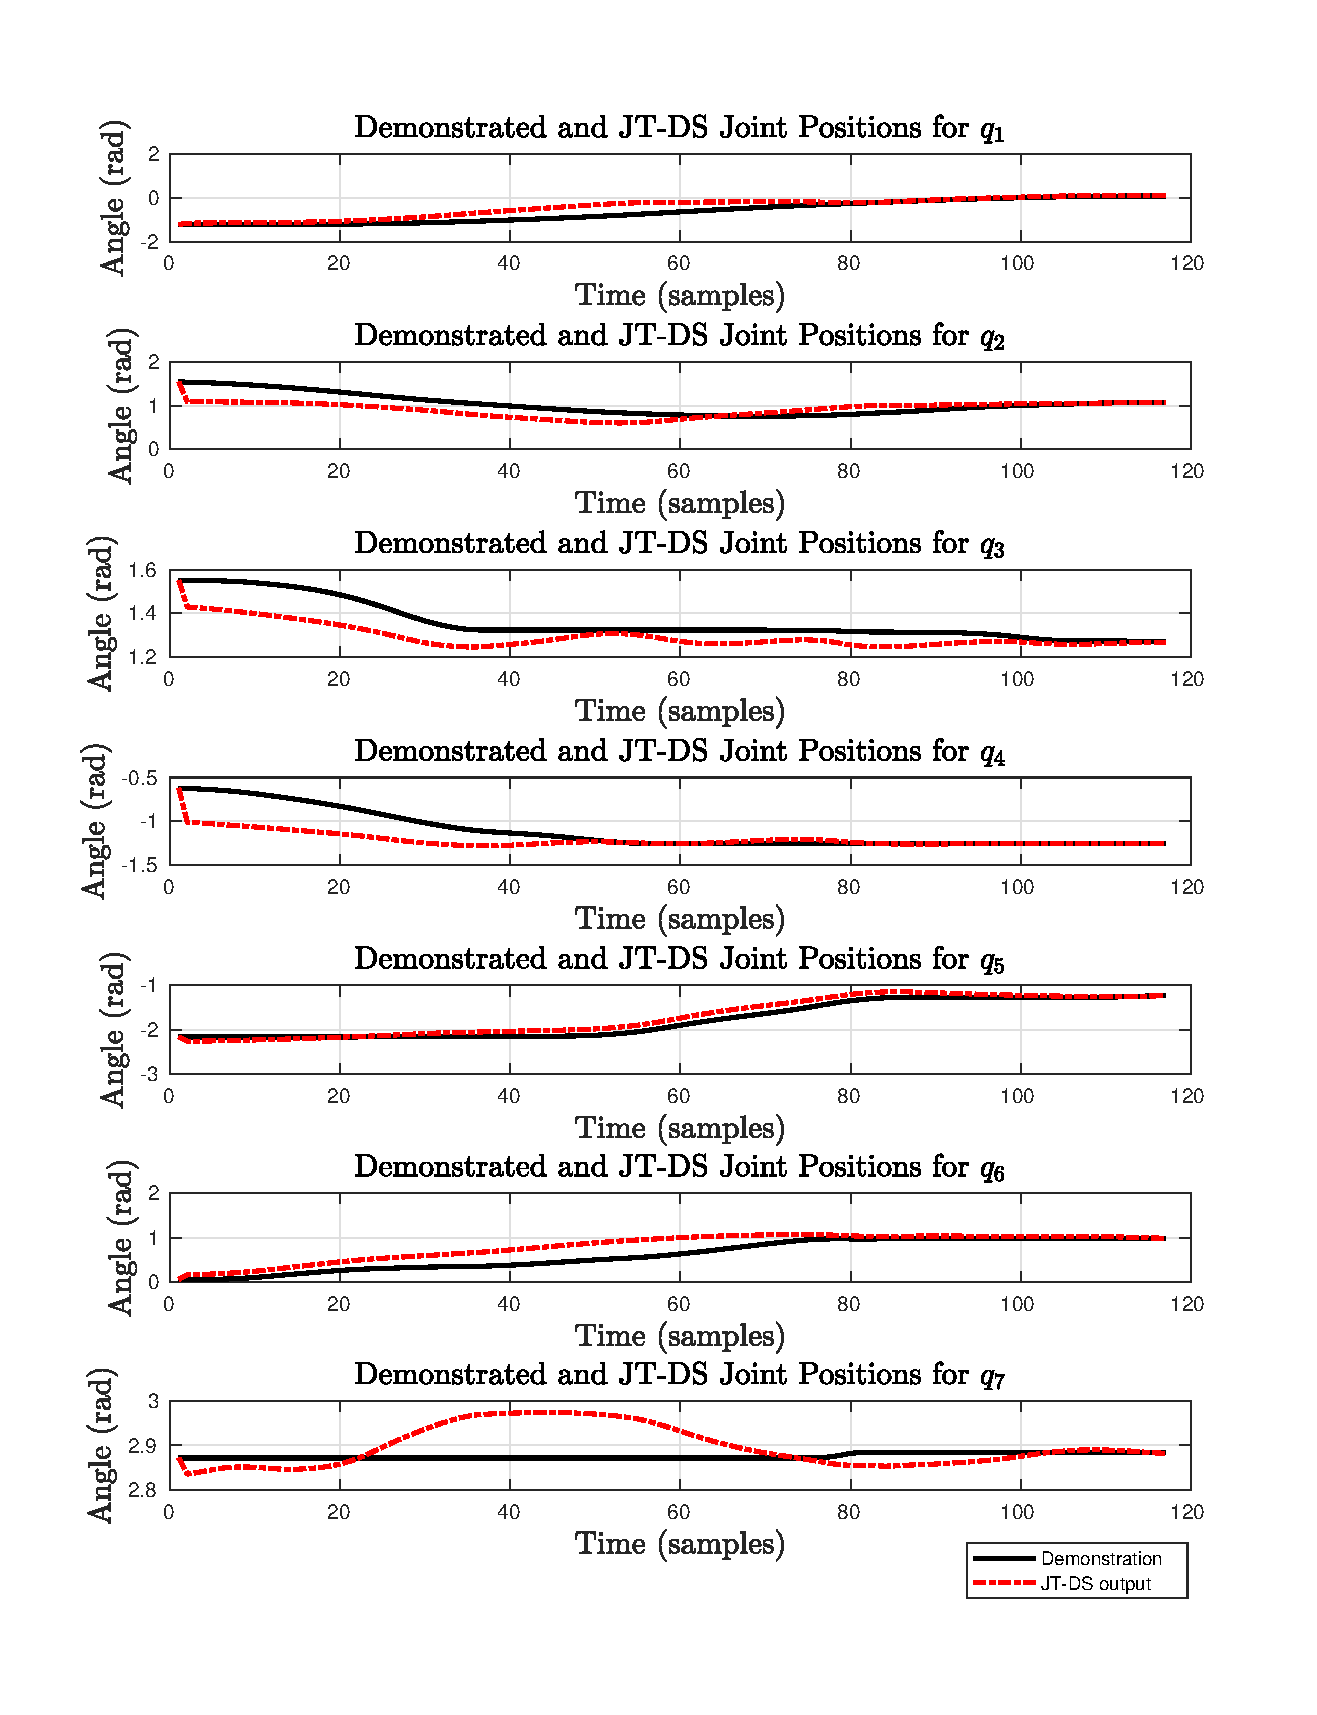
\includegraphics[trim={1.2cm 1.5cm 1.7cm 1.5cm},clip,width=\linewidth]{../../src/JTDS_mat_lib/figures/jtd_pos_pour1.pdf}
  \end{minipage}
    \begin{minipage}{0.5\textwidth}
       	\centering 
       	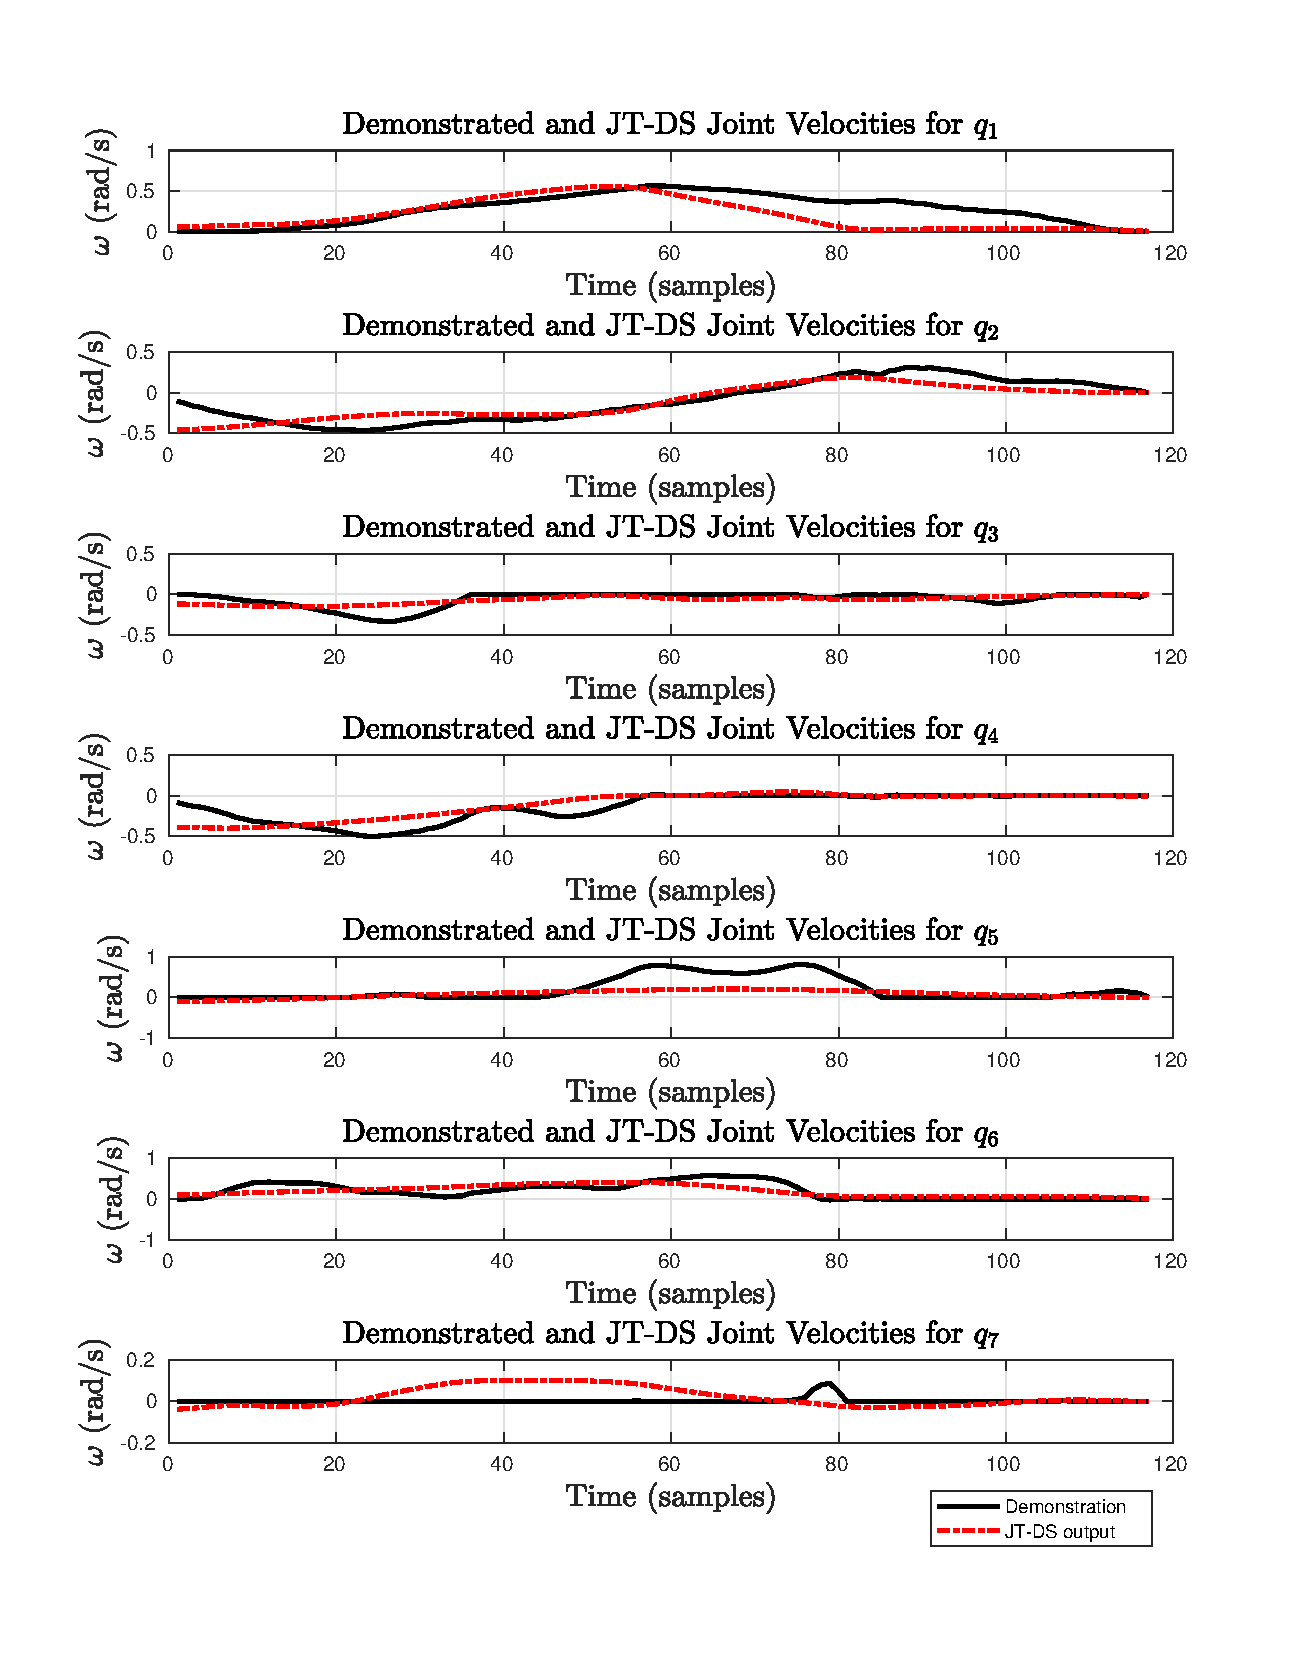
\includegraphics[trim={1.2cm 1.5cm 1.7cm 1.5cm},clip,width=\linewidth]{../../src/JTDS_mat_lib/figures/jtd_vel_pour1.pdf}
    \end{minipage}
   \caption{Training and executed joint-position/velocities with JT-DS for 1 pouring demonstrations. \label{fig:jtds_velocities}}
\end{figure*}

Note that our controller is not generating the entire trajectory in one-shot, it is generating the next desired velocity given the current joint posture, e.g. $\dot{q}_{t+1} = \mathcal{A}(q_{t})J^T(q_{t})(H(q_{t})-x^*)$ with $q_t$ being the current joint configuration. Moreover, our controller is state-dependent only; i.e. it has no dependence on time or the duration of the desired trajectories. Hence, it can generate motions similar to the demonstrated ones at different frequencies and time durations. \\

\noindent \underline{On the applicability of F-PCA to our learning scheme:}  If we were to ignore our proposed control scheme and try to reconstruct the trajectories from the joint postural synergy components; i.e. using PCA, we would get the trajectories shown in Fig. \ref{fig:pca_velocities}. In these plots, we are taking one of the collected demonstrations projected in the PCA-space, i.e. $\phi(\{q_1,q_2,\dots,q_T\})$ and reconstructing it to generate the desired joint posture trajectories. To compute the velocities we apply numerical differentiation on the reconstructed joint positions. As can be seen, we are capable of generating similar trajectories, both in position and velocity. In this simple example we are saving the entire demonstration in PCA-space, however, if we were to use this for controlling the real robot we need to learn a model or a controller in this low-dimensional space and then map it back to joint-space. As discussed earlier, this is not feasible with our proposed control-law \eqref{eq:jtds}, due to the stability and convergence objectives we defined. 

\begin{figure*}[!th] 
  \begin{minipage}{0.485\textwidth}
     	\centering 
     	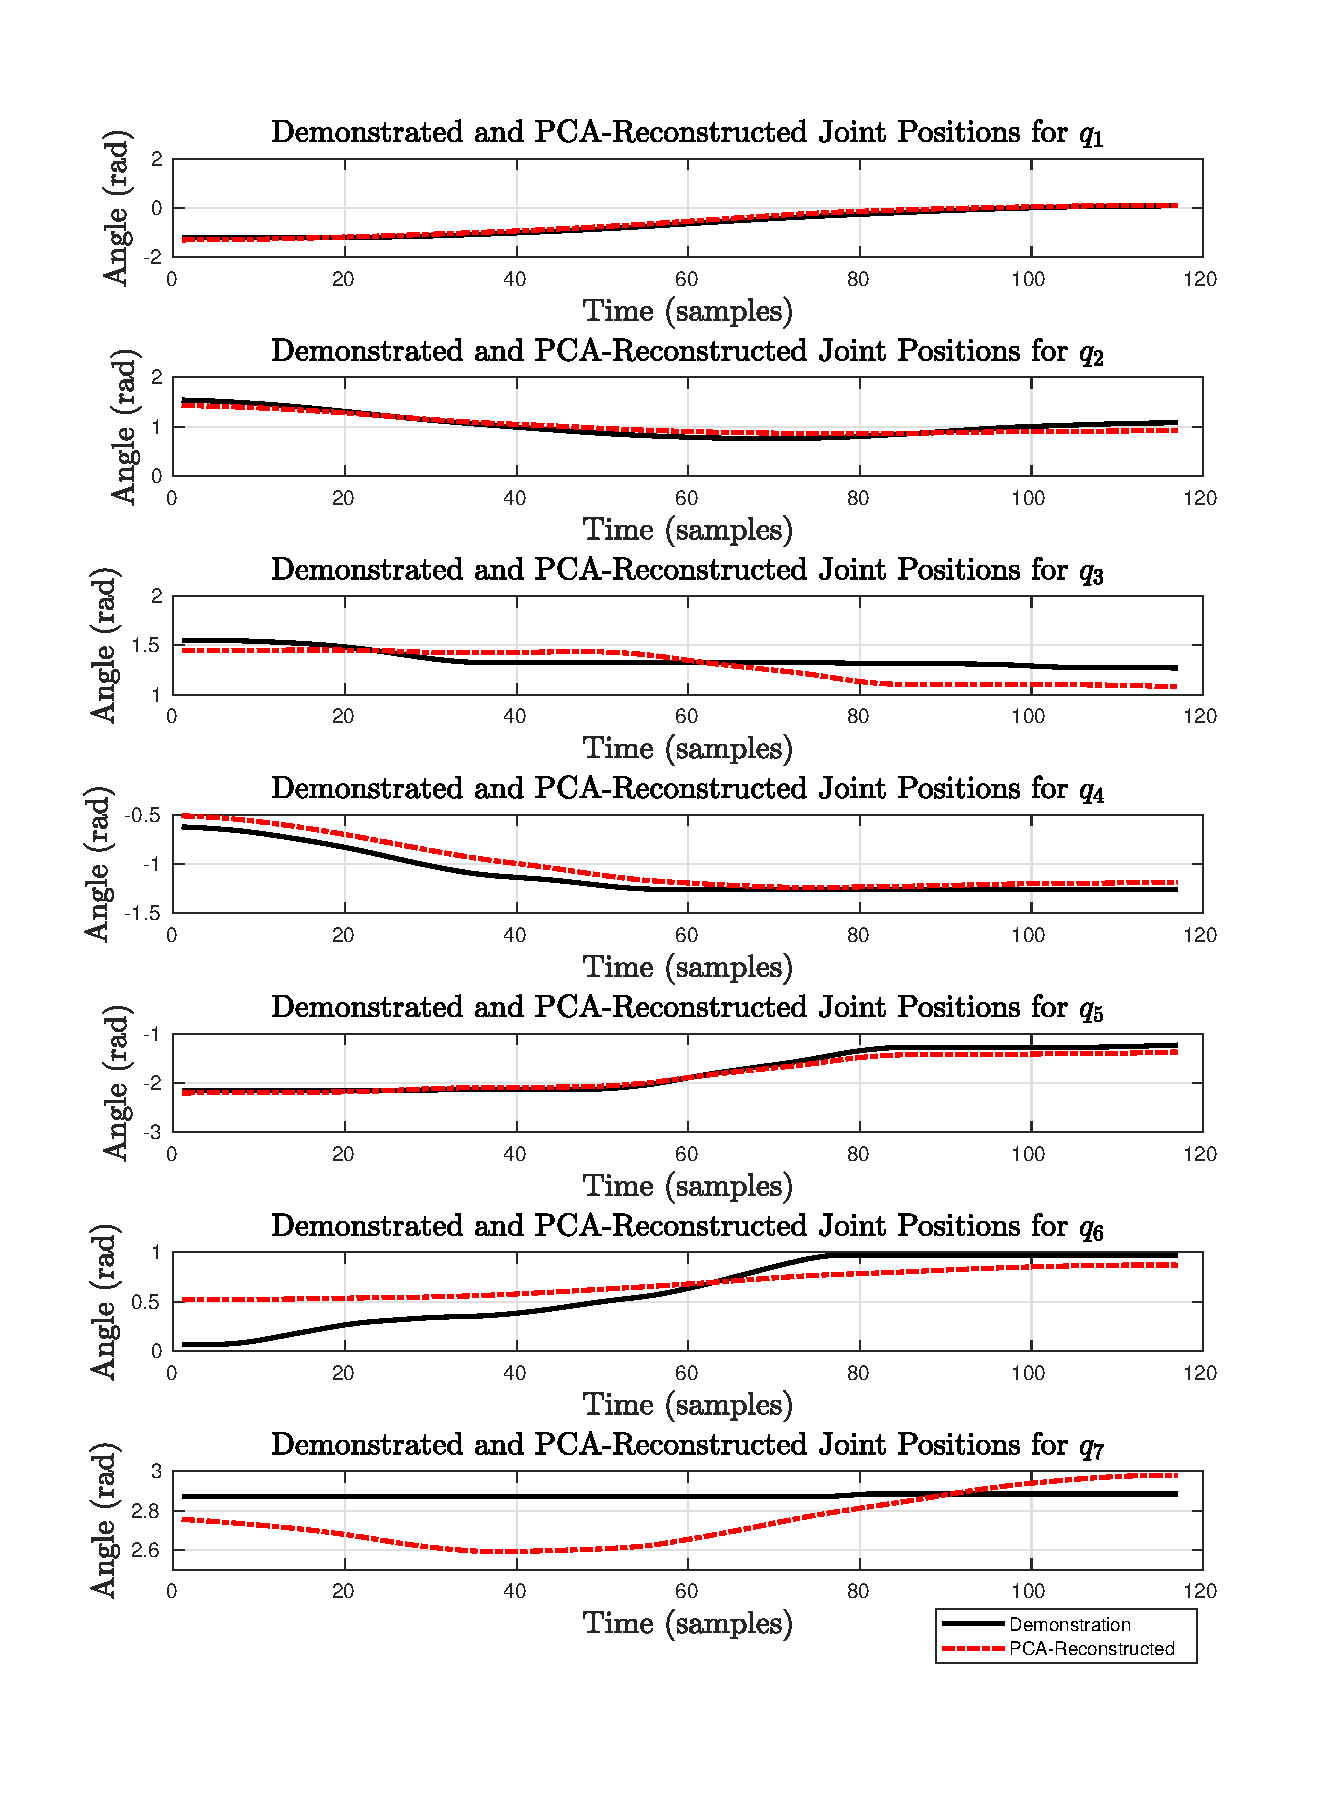
\includegraphics[trim={1.2cm 1.5cm 1.7cm 1.5cm},clip,width=\linewidth]{../../src/JTDS_mat_lib/figures/pca_pos_pour1.pdf}
  \end{minipage}
    \begin{minipage}{0.5\textwidth}
       	\centering 
       	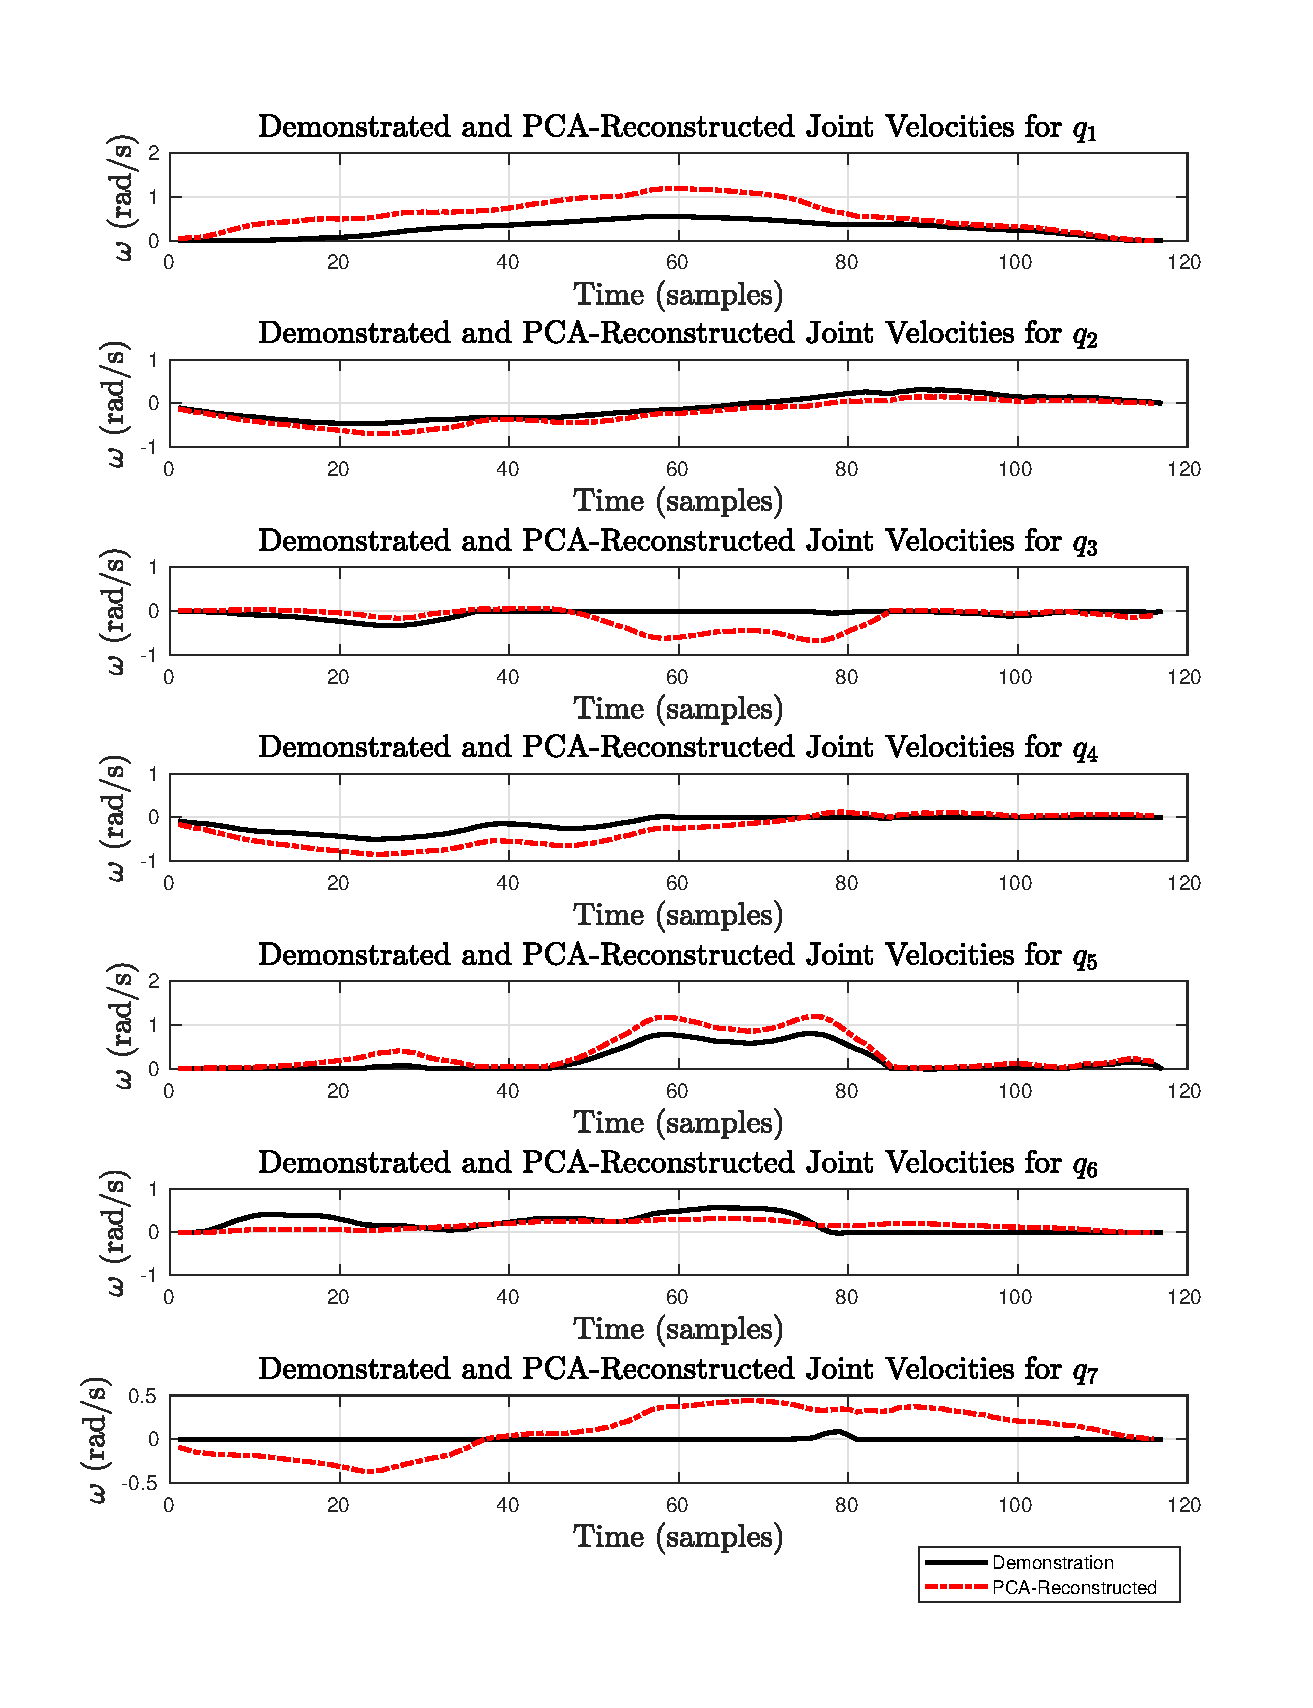
\includegraphics[trim={1.2cm 1.6cm 1.7cm 1.6cm},clip,width=\linewidth]{../../src/JTDS_mat_lib/figures/pca_vel_pour1.pdf}
    \end{minipage}
   \caption{Training and reconstructed joint-position/velocities with PCA for 1 pouring demonstrations. \label{fig:pca_velocities}}
\end{figure*}

Ignoring our limitation, one of the main draw-backs of this type of synergistic control is that the extracted representation in PCA space does not take into account the dynamic features of the motions and further assumes that the demonstrations have no time correlation. As mentioned by the reviewer and applied in \cite{Dai:IROS:2013} for modeling grasping motions and in \cite{Averta:FRAI:2017} for upper-limb motions, functional-PCA is a nice alternative to include these dynamic features and further reconstruct entire trajectories with a linear combination of a few \textit{time-dependent} functions. In this approach each demonstrated trajectory (of a single DOF) is considered as a function composed of a linear combination of $N$ basis elements (which can ve exponentials, splines, Fourier) $f_i = \sum\limits_{n=1}^{N}\theta_nb_N$. Thus, each $i$-th function (i.e. $i$-th demonstration) can be described by the vector a coefficients $\Theta = \{\theta_1,\dots,\theta_N\}$. PCA is then performed on $\Theta = \{\theta_1,\dots,\theta_N\}$ and the extracted PC are transformed to \textit{functional PCs} via the $N$ basis functions. Then $M<N$ \textit{functional PCs} are used to reconstruct the $i$-th function (i.e. $i$-th demonstration ) as $\hat{f}_i = \bar{f_i} + \sum\limits_{i=1}^{M}c_i\xi_i$, where $\bar{f}_i$ is the mean function, $c_i$ are the coefficients and $\xi_i$ are the \textit{functional PCs}. As shown in \cite{Averta:FRAI:2017} with only 1 \textit{functional PCs} 60/70\% of the demonstrations can be accurately reconstructed. This approach would be interesting if our goal were to reconstruct entire time-dependent trajectories as they do in  \cite{Dai:IROS:2013} and \cite{Averta:FRAI:2017}. This is, however, NOT our goal and applying this method to our control scheme seems not suitable and is rather an alternative approach for the following reasons: First of all, in this work we propose a DS-based controller, meaning that, we do not generate the full reference trajectory of the robot \textit{a prior} and then try to track it, we instead compute the next desired velocity on-the-fly which happens to result in the desired motion because it is encoded in $\mathcal{A}(q)$. Second, if we were to apply this method as the reviewer suggests, the only way to do it is to re-write a controller that uses 7 reconstructed functions $\hat{f}_i$ (i.e. one per joint) to track a time-indexed reference joint trajectory. This is a valid approach, however, in this work we propose a state-dependent; i.e. time-invariant approach. Finally, our goal not to accurately reproduce the demonstrations but rather to reach the target $x^*$ with a similar joint motion as the one that was demonstrated.

\bibliographystyle{plain}
\bibliography{Refs.bib}

\end{document}

